\chapter{i-vectorの抽出精度向上のための発話区間結合手法}
\label{chapter:prob_method}
\ref{section:pre_cos}節で述べたように、i-vectorは発話ができるだけ長いほうが正確に話者の特徴を抽出することができる。そこで、時系列順に並んでいる発話区間のうち、発話から得られるi-vectorを用いて前後の発話が同一話者である可能性が高い発話区間を結合し、擬似的に長い発話を作成することでi-vectorの抽出精度の向上が見込めると考えた。しかし、非常に短い発話からはi-vectorが十分に抽出できないため、コサイン類似度のみを用いた場合、異なる話者同士の発話区間を結合する可能性がある。そのため本稿では「発話間の時間情報」「発話環境」に着目し、2通りの手法で発話区間を結合した。1つ目は発話間の時間情報を考慮した発話区間の結合手法である。2つめは、話者の発話環境を考慮した発話区間の結合手法である。図\ref{fig:indexing2}は、本稿の提案手法を組み込んだインデクシング手法の流れである。

\begin{figure}[H]
  \begin{center}
    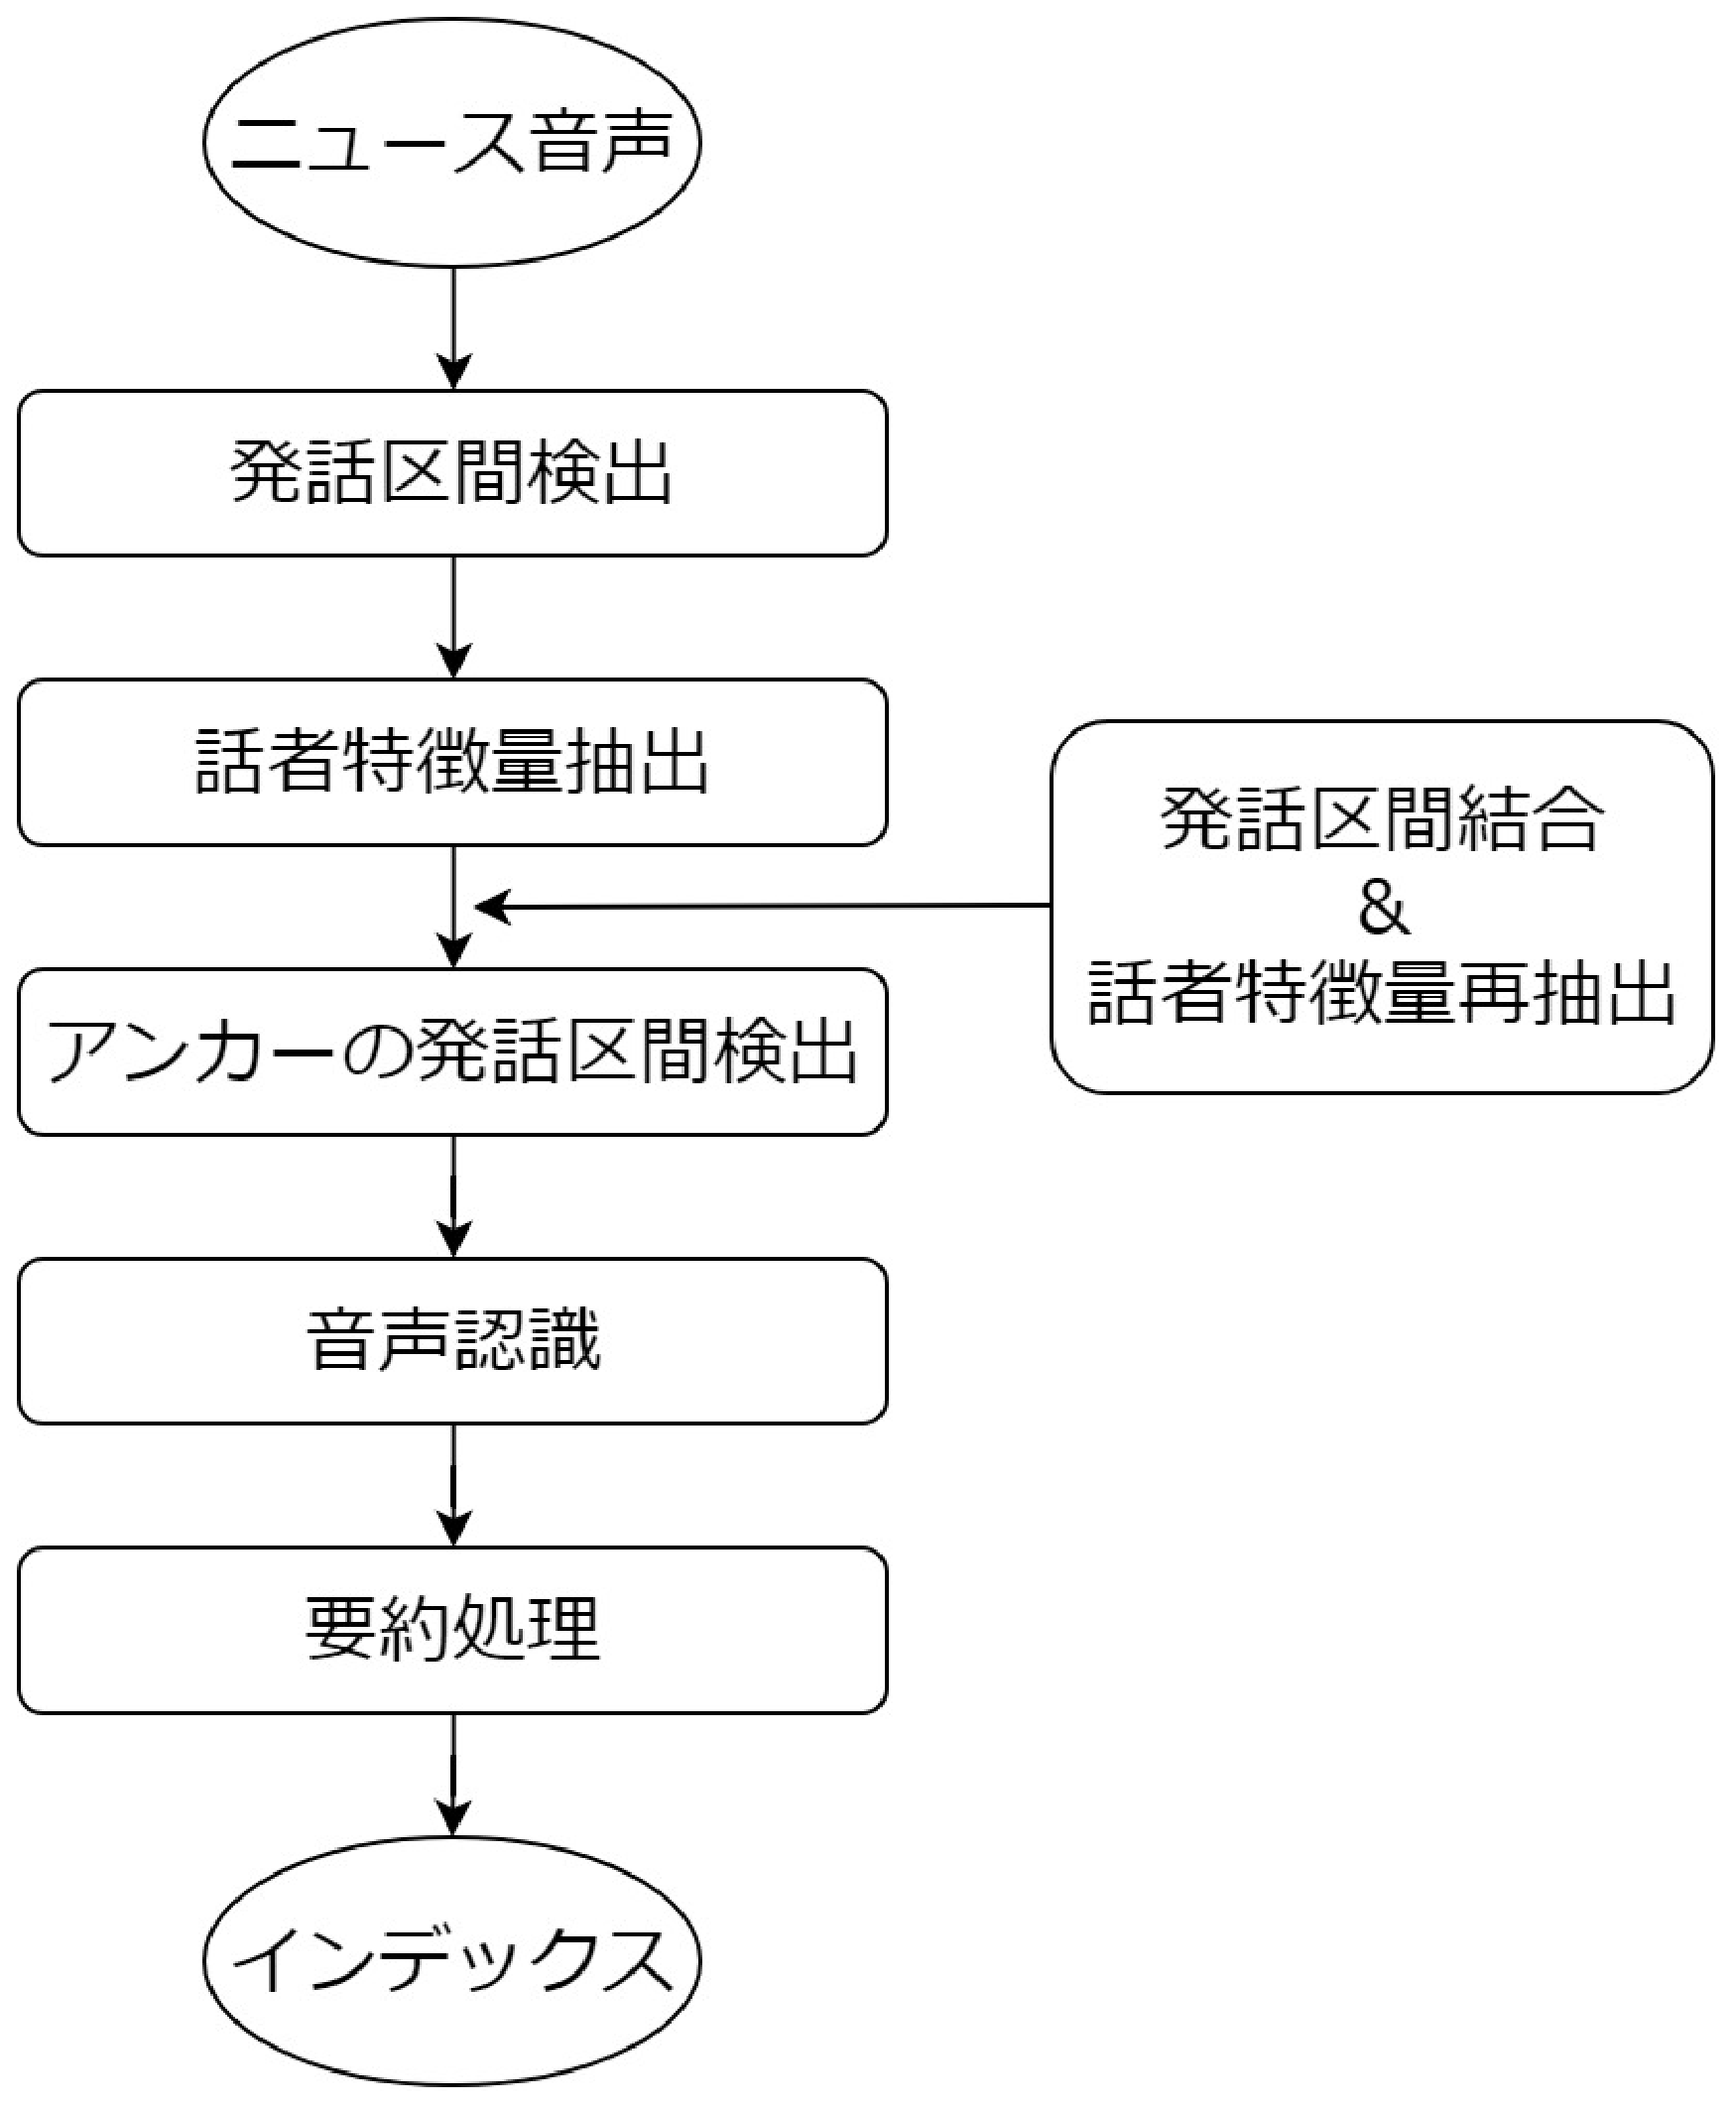
\includegraphics[scale=0.3]{./figure/indexing2.eps}
  \end{center}
  \caption{提案手法を組み込んだインデクシング手法 \label{fig:indexing2}}
\end{figure}

\section{発話間の時間情報を考慮した発話区間の結合手法}
本手法では、発話区間と発話区間の間(非発話区間)が短い場合、発話区間を結合する。これは図\ref{fig:same_sp}で示されるように、同一話者が連続で発話する場合は間をおかずに次の発話を行うことが非常に多いためである。つまり、非発話区間が非常に短いとき、高い確率で同一話者の発話が行われる。そこで、非発話区間が非常に短い場合、同一話者の発話と判別し発話区間を結合する。

\section{発話環境を考慮した発話区間の結合手法}
本手法では発話環境を音源識別によって検出し、発話環境の変化を検出した場合、同一話者の可能性が高いとして前後の発話区間を結合する。ニュース番組にはスタジオにいるアンカーのほか、台風の状況を中継する中継アナウンサー、騒音の中でインタビューを受けるインタビューイなどが存在する。例えば、アンカーから中継アナウンサー、インタビューイからアンカーなど話者が切り替わった場合、発話環境が変化する。本稿で使用する音源識別システムはニュース番組音声を「音声」「背景雑音」「音楽」「無音」のいずれかに分類する。そのため、「音声」以外の区間、つまり非発話区間の音源識別結果である「背景雑音」「音楽」「無音」の検出結果が変化した時発話環境の変化したと識別することができる。これらより、発話環境が変化するまでの範囲で発話している話者を同一話者として発話区間を結合する。\par
